\section{Simulink}

Simulink is a commercial modelling and simulation tool developed by MathWorks. It is an industry standard in the field of control engineering. Models are created graphically in a block-based user interface and simulation results can be easily be analysis with plots or mode advanced tools. Additionally a large number of internal and third-party libraries further simplify modelling, especially in specialized fields such a music or aerospace.

Simulink is also tightly integrated in MATLAB, MathWorks' commercial numerical computation tool, which is widely used in academia and industry in many different fields. Simulink runs inside the MATLAB environment and can thus easily be controlled, tested or extended using the MATLAB programming language.

\begin{figure}[simulink_screenshot]
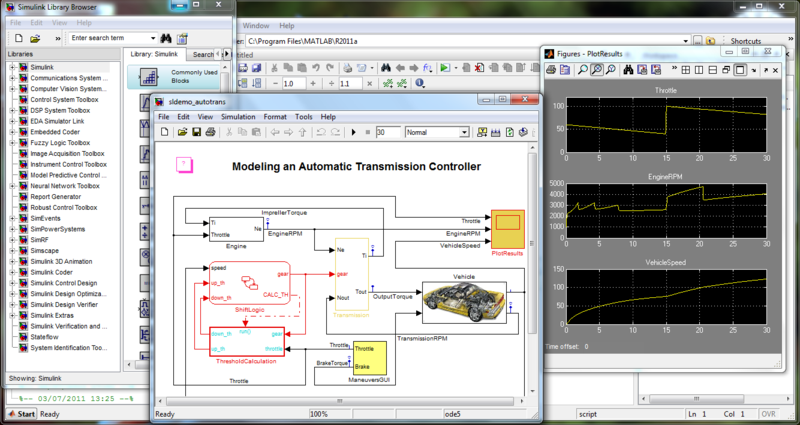
\includegraphics[width=16cm]{media/simulink_screenshot.png}
% \includegraphics*[width=0.38\textwidth]{media/ETH_logo} \hfill
\caption{Screenshot of Simulink}
\label{simulink_screenshot}
\end{figure}

Simulink is especially useful for engineers because no programming knowledge is required even for modelling complex dynamic systems (example: power plants). Default configuration options and an entirely graphical interface hide most implementation details (simulation details, solver types, et). A graphical modelling interface is also useful because it allows a more intuitive understanding of the model, unlike the large mathematical matrices used in Markov Chains, Markov Decision Processes or Partially Observable Markov Decision Processes.

Figure~\ref{simulink_screenshot} shows an example of the MATLAB environment, a Simulink model and plots of simulation results.
